\documentclass[12pt,a4paper]{scrartcl}
\author{Lecture: Martin Hering-Betram}
\usepackage[english]{babel}
\usepackage[none]{hyphenat}
\usepackage[T1]{fontenc}
\usepackage{graphicx, subfig}
\graphicspath{{img/}}
\usepackage[document]{ragged2e}
\usepackage{lmodern}
\usepackage{color}
\usepackage{amsmath}
\usepackage{graphicx}
 
\title{Delivery of computer graphics}
\date{18. April 2018}

\begin{document}


\maketitle

\begin{center}

\Large
\textbf{Studiengang:} Medieninformatik
\\
\textbf{Fachsemester:} 4
\\[3cm]
\textbf {Autoren:}
\\Fabian Niehaus
\\501297
\\Tuyet Nguyen
\\5009445

\end{center}
\newpage
\Large
\tableofcontents
\newpage
\Large
\vspace{3cm}
\section{Excercise 1}

\subsection{Problem 1: Rendering Quad Meshes}

\large
\textbf{Problem} \\
-Develop a class Vertex and a class Quad. The Vertex class may contain three coordinates and the
valence (number of edges). The Quad class may contain the indices of four vertices and of four
adjacent quads. Normal vectors can be calculated from the cross product between two diagonals.\\
-Implement a function to read points and faces from OBJ. You can assume that all faces are quads (for an example, see cube.obj). Since the number of vertices and quads is not known before reading the file, static arrays are not a good choice. Instead, vectors may be used: vector vertices; vector quads;\\
-Implement a function drawing the mesh c1 as quadrilateral polygons and c2 as wireframe, using GLQUADS (with normal vectors and lighting) and GLLINES (without lighting), respectively.\\[0,5cm]

\textbf{Approach}\\
To solve the problems we used OpenGL and QT Creator. In the program QT the Vertex class and Quad class are created.\\
The vertex class contains the information of three x,y,z coordinates and the valence. In the Quads class has the four edges vertices and of four adjacent.\\
For the next task, the points and faces are to be read from the file Cube.obj with the help of the "pushback" method. The file Cube is predefined. \\
Two squares are created for the last task. There are quadrilateral polygons and as wireframe..The oglwidget and oglwidget2 class are defined here.There two can be showed on diffirent windows. This step can be done with mainwindown.ui.\\
We used a "for" loop here. The methods in "for" loop read the points and connect the points with the lines(polygons) .And we used the same methos for the 3D Object (wireframe)\\[0,5cm]

\newpage

\textbf{Implementation}\\


Vertex define --> vertex.cpp\\
Quad define --> quad.cpp\\
read points and faces --> oglwidget2.cpp / line 3\\
draw quad --> oglwidget2.cpp / line 37 to 64\\
draw 3D-quad --> oglwidget2.cpp / line 72 to 90\\
SetMaterialColor --> oglwidget2.cpp / line 109 to 132\\
InitLightingAndProjection --> oglwidget2.cpp / line 133 to 166\\
initializeGL() --> line 167 to 183\\
paintGL --> line 185 to 210\\
resizeGL --> line 212 to 216 \\[0,5cm]



\textbf{Result}\\

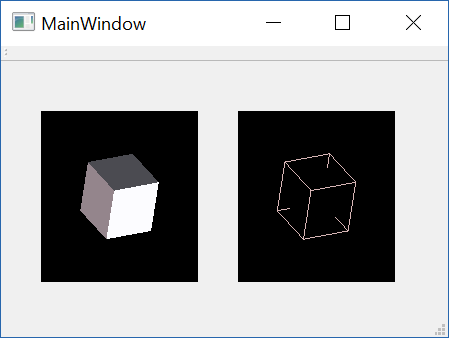
\includegraphics[width=0.7\textwidth]{Problem 1.png}\\

\subsection{Problem 2: Mesh Connectivity}

\large
\textbf{Problem}\\
-Implement a function calculating the vertex valences and connecting each quad to its neighbors.
You can assume that the mesh does not have boundaries, i.e. every quad has four neighbors.\\
-Print the entire data structure on the screen (or into a file). Devise and perform tests to validate
its correctness.\\
The mesh connectivity provides the basis for Catmull-Clark subdivision, which will be subject of the
next assignment.\\[0,5cm]
\textbf{Approach}\\
We have taken the following steps in this task.\\
+) We have a method to count the edge.\\
+) Then a method was created to search for the edge neighbours. The method takes a square and then looks for each of the 4 edges of this square, if any other square divides this edge, respectively these 2 corner points.\\[0,5cm]
\textbf{Implementation}\\
calculateVertexValence--> oglwidget.cpp / line 109 to 139\\
compareVertices --> vertex.cpp / line 51 to 61\\
determineQuadNeighbours --> oglwidget.cpp / line 143 to 178\\[0,5cm]
\textbf{Results}\\

Eckpunkte: 2|14|8|17| - Nachbarn: 23|1|3|10\\
Eckpunkte: 3|15|8|14| - Nachbarn: 13|2|0|22\\
Eckpunkte: 1|16|8|15| - Nachbarn: 17|3|1|12\\
Eckpunkte: 0|17|8|16| - Nachbarn: 11|0|2|16\\
Eckpunkte: 4|18|9|21| - Nachbarn: 19|5|7|8\\
Eckpunkte: 5|19|9|18| - Nachbarn: 15|6|4|18\\
Eckpunkte: 7|20|9|19| - Nachbarn: 21|7|5|14\\
Eckpunkte: 6|21|9|20| - Nachbarn: 9|4|6|20\\
Eckpunkte: 4|21|10|23| - Nachbarn: 4|9|11|19\\
Eckpunkte: 6|22|10|21| - Nachbarn: 20|10|8|7\\
Eckpunkte: 2|17|10|22| - Nachbarn: 0|11|9|23\\
Eckpunkte: 0|23|10|17| - Nachbarn: 16|8|10|3\\
Eckpunkte: 1|15|11|25| - Nachbarn: 2|13|15|17\\
Eckpunkte: 3|24|11|15| - Nachbarn: 22|14|12|1\\
Eckpunkte: 7|19|11|24| - Nachbarn: 6|15|13|21\\
Eckpunkte: 5|25|11|19| - Nachbarn: 18|12|14|5\\
Eckpunkte: 0|16|12|23| - Nachbarn: 3|17|19|11\\
Eckpunkte: 1|25|12|16| - Nachbarn: 12|18|16|2\\
Eckpunkte: 5|18|12|25| - Nachbarn: 5|19|17|15\\
Eckpunkte: 4|23|12|18| - Nachbarn: 8|16|18|4\\
Eckpunkte: 6|20|13|22| - Nachbarn: 7|21|23|9\\
Eckpunkte: 7|24|13|20| - Nachbarn: 14|22|20|6\\
Eckpunkte: 3|14|13|24| - Nachbarn: 1|23|21|13\\
Eckpunkte: 2|22|13|14| - Nachbarn: 10|20|22|0\\
Eckpunkte: 2|14|8|17| - Nachbarn: 23|1|3|10\\
Eckpunkte: 3|15|8|14| - Nachbarn: 13|2|0|22\\
Eckpunkte: 1|16|8|15| - Nachbarn: 17|3|1|12\\
Eckpunkte: 0|17|8|16| - Nachbarn: 11|0|2|16\\
Eckpunkte: 4|18|9|21| - Nachbarn: 19|5|7|8\\
Eckpunkte: 5|19|9|18| - Nachbarn: 15|6|4|18\\
Eckpunkte: 7|20|9|19| - Nachbarn: 21|7|5|14\\
Eckpunkte: 6|21|9|20| - Nachbarn: 9|4|6|20\\
Eckpunkte: 4|21|10|23| - Nachbarn: 4|9|11|19\\
Eckpunkte: 6|22|10|21| - Nachbarn: 20|10|8|7\\
Eckpunkte: 2|17|10|22| - Nachbarn: 0|11|9|23\\
Eckpunkte: 0|23|10|17| - Nachbarn: 16|8|10|3\\
Eckpunkte: 1|15|11|25| - Nachbarn: 2|13|15|17\\
Eckpunkte: 3|24|11|15| - Nachbarn: 22|14|12|1\\
Eckpunkte: 7|19|11|24| - Nachbarn: 6|15|13|21\\
Eckpunkte: 5|25|11|19| - Nachbarn: 18|12|14|5\\
Eckpunkte: 0|16|12|23| - Nachbarn: 3|17|19|11\\
Eckpunkte: 1|25|12|16| - Nachbarn: 12|18|16|2\\
Eckpunkte: 5|18|12|25| - Nachbarn: 5|19|17|15\\
Eckpunkte: 4|23|12|18| - Nachbarn: 8|16|18|4\\
Eckpunkte: 6|20|13|22| - Nachbarn: 7|21|23|9\\
Eckpunkte: 7|24|13|20| - Nachbarn: 14|22|20|6\\
Eckpunkte: 3|14|13|24| - Nachbarn: 1|23|21|13\\
Eckpunkte: 2|22|13|14| - Nachbarn: 10|20|22|0\\

\newpage

\section{Excercise 2}

\subsection{Problem 1: Catmull-Clack Subdivision Masks}

\large
\textbf{Problem}\\
- Implement the face subdivision mask (f = durchschnitt von v(f)) computing the midpoint of each quad and adding it to the vertex vector\\
- Based on the mesh connectivity structure from exercise 1, find a way to computer and add the edge vertices to the vertex vector\\
- Implement the vertex mask, modifying the original vertices\\
 
\textbf{Approach}\\
\textbf{Implementation}\\
\textbf{Results}\\
\subsection{Problem 2: Recursive Subdivision}

\large
\textbf{Problem}\\
Replace every face by the four sub-faces connected to the correct vertices. Restore the mesh
connectivity and apply two more subdivisions before rendering. \\
\textbf{Approach}\\
The method subdivideAndReconnectMesh is provided. The function builds a square of one point with two its edge point and one face point.\\
\textbf{Implementation}\\
subdivideAndReconnectMesh --> oglwidget /Line 256 to 280\\
\textbf{Results}\\

\end{document}
